\documentclass[twoside]{book}

% Packages required by doxygen
\usepackage{calc}
\usepackage{doxygen}
\usepackage{graphicx}
\usepackage[utf8]{inputenc}
\usepackage{makeidx}
\usepackage{multicol}
\usepackage{multirow}
\usepackage{textcomp}
\usepackage[table]{xcolor}

% Font selection
\usepackage[T1]{fontenc}
\usepackage{mathptmx}
\usepackage[scaled=.90]{helvet}
\usepackage{courier}
\usepackage{amssymb}
\usepackage{sectsty}
\renewcommand{\familydefault}{\sfdefault}
\allsectionsfont{%
  \fontseries{bc}\selectfont%
  \color{darkgray}%
}
\renewcommand{\DoxyLabelFont}{%
  \fontseries{bc}\selectfont%
  \color{darkgray}%
}

% Page & text layout
\usepackage{geometry}
\geometry{%
  a4paper,%
  top=2.5cm,%
  bottom=2.5cm,%
  left=2.5cm,%
  right=2.5cm%
}
\tolerance=750
\hfuzz=15pt
\hbadness=750
\setlength{\emergencystretch}{15pt}
\setlength{\parindent}{0cm}
\setlength{\parskip}{0.2cm}
\makeatletter
\renewcommand{\paragraph}{%
  \@startsection{paragraph}{4}{0ex}{-1.0ex}{1.0ex}{%
    \normalfont\normalsize\bfseries\SS@parafont%
  }%
}
\renewcommand{\subparagraph}{%
  \@startsection{subparagraph}{5}{0ex}{-1.0ex}{1.0ex}{%
    \normalfont\normalsize\bfseries\SS@subparafont%
  }%
}
\makeatother

% Headers & footers
\usepackage{fancyhdr}
\pagestyle{fancyplain}
\fancyhead[LE]{\fancyplain{}{\bfseries\thepage}}
\fancyhead[CE]{\fancyplain{}{}}
\fancyhead[RE]{\fancyplain{}{\bfseries\leftmark}}
\fancyhead[LO]{\fancyplain{}{\bfseries\rightmark}}
\fancyhead[CO]{\fancyplain{}{}}
\fancyhead[RO]{\fancyplain{}{\bfseries\thepage}}
\fancyfoot[LE]{\fancyplain{}{}}
\fancyfoot[CE]{\fancyplain{}{}}
\fancyfoot[RE]{\fancyplain{}{\bfseries\scriptsize Generated on Sat Jun 14 2014 22\-:06\-:12 for E\-K\-U\-L\-M\-S by Doxygen }}
\fancyfoot[LO]{\fancyplain{}{\bfseries\scriptsize Generated on Sat Jun 14 2014 22\-:06\-:12 for E\-K\-U\-L\-M\-S by Doxygen }}
\fancyfoot[CO]{\fancyplain{}{}}
\fancyfoot[RO]{\fancyplain{}{}}
\renewcommand{\footrulewidth}{0.4pt}
\renewcommand{\chaptermark}[1]{%
  \markboth{#1}{}%
}
\renewcommand{\sectionmark}[1]{%
  \markright{\thesection\ #1}%
}

% Indices & bibliography
\usepackage{natbib}
\usepackage[titles]{tocloft}
\setcounter{tocdepth}{3}
\setcounter{secnumdepth}{5}
\makeindex

% Hyperlinks (required, but should be loaded last)
\usepackage{ifpdf}
\ifpdf
  \usepackage[pdftex,pagebackref=true]{hyperref}
\else
  \usepackage[ps2pdf,pagebackref=true]{hyperref}
\fi
\hypersetup{%
  colorlinks=true,%
  linkcolor=blue,%
  citecolor=blue,%
  unicode%
}

% Custom commands
\newcommand{\clearemptydoublepage}{%
  \newpage{\pagestyle{empty}\cleardoublepage}%
}


%===== C O N T E N T S =====

\begin{document}

% Titlepage & ToC
\hypersetup{pageanchor=false}
\pagenumbering{roman}
\begin{titlepage}
\vspace*{7cm}
\begin{center}%
{\Large E\-K\-U\-L\-M\-S }\\
\vspace*{1cm}
{\large Generated by Doxygen 1.8.6}\\
\vspace*{0.5cm}
{\small Sat Jun 14 2014 22:06:12}\\
\end{center}
\end{titlepage}
\clearemptydoublepage
\tableofcontents
\clearemptydoublepage
\pagenumbering{arabic}
\hypersetup{pageanchor=true}

%--- Begin generated contents ---
\chapter{Readme}
\label{md__readme}
\hypertarget{md__readme}{}
\#\-E\-K\-U\-L\-M\-S

\subsection*{Readme}

The goal of this project is to create a Learning Management System suited for the specific needs of Eastern Kentucky University, specifically (for now) the Computer Science department. This is part of an undergraduate research project into the current state of Learning Management Systems and how they can be better improved to support student learning.

As of April 8th, 2014, E\-K\-U\-L\-M\-S is in alpha stage. This is a proof of concept that focuses on basic functions for creating tests and courses, and allowing users to track their progress. After April 28th, 2014, E\-K\-U\-L\-M\-S will undergo a major overhaul in code quality and usability.

\subsubsection*{Features to be completed at launch (Beginning of Fall 2014 semester)}


\begin{DoxyItemize}
\item Basic user account management -\/ {\bfseries Complete}
\item Basic course management -\/ {\bfseries Complete}
\item Basic test management -\/ {\bfseries In progress}
\item Integration with the E\-K\-U Central Authentication System -\/ {\bfseries Todo}
\item My\-S\-Q\-L P\-D\-O queries instead of inline P\-H\-P -\/ {\bfseries Todo}
\item User statistics with visual graphs representing a student's progress over time -\/ {\bfseries In progress}
\item Aesthetically pleasing, functional, and user-\/friendly U\-I -\/ {\bfseries Todo}
\item Complete A\-J\-A\-X/\-J\-S\-O\-N based R\-E\-S\-T A\-P\-I -\/ Indefinitely in progress$\ast$$\ast$
\item Full P\-H\-P\-Doc documentation for ease of future development -\/ {\bfseries Indefinitely in progress}
\item Complete code refactor to provide clean, maintainable code -\/ {\bfseries Todo}
\item Setup and migration scripts (Python or P\-H\-P) -\/ {\bfseries Todo (not necessary for launch)}
\item Full H\-T\-M\-L5 web standards compliance -\/ {\bfseries Indefinitely in progress}
\item Full responsive design -\/ {\bfseries Todo (not necessary for launch)}
\end{DoxyItemize}

\subsubsection*{Possible features to be implemented in the future}


\begin{DoxyItemize}
\item Short video tutorials per test
\item Tutorials with autocomplete search and smart suggestions (this is very unlikely in the near future)
\item Questions where the user will have to code and said code will be evaluated for correctness
\item Anything else that is requested, within reason
\end{DoxyItemize}

Again, this is currently in very rough, incomplete Alpha stage and is not completely indicative of what will be available at launch 
\chapter{Todo List}
\label{todo}
\hypertarget{todo}{}

\begin{DoxyRefList}
\item[\label{todo__todo000008}%
\hypertarget{todo__todo000008}{}%
Class \hyperlink{class_courses}{Courses} ]make a function to check if a course already exists 
\end{DoxyRefList}
\chapter{Hierarchical Index}
\section{Class Hierarchy}
This inheritance list is sorted roughly, but not completely, alphabetically\-:\begin{DoxyCompactList}
\item \contentsline{section}{Db}{\pageref{class_db}}{}
\begin{DoxyCompactList}
\item \contentsline{section}{Users}{\pageref{class_users}}{}
\begin{DoxyCompactList}
\item \contentsline{section}{Courses}{\pageref{class_courses}}{}
\begin{DoxyCompactList}
\item \contentsline{section}{Tests}{\pageref{class_tests}}{}
\end{DoxyCompactList}
\end{DoxyCompactList}
\end{DoxyCompactList}
\end{DoxyCompactList}

\chapter{Data Structure Index}
\section{Data Structures}
Here are the data structures with brief descriptions\-:\begin{DoxyCompactList}
\item\contentsline{section}{\hyperlink{class_courses}{Courses} }{\pageref{class_courses}}{}
\item\contentsline{section}{\hyperlink{class_db}{Db} }{\pageref{class_db}}{}
\item\contentsline{section}{\hyperlink{class_tests}{Tests} }{\pageref{class_tests}}{}
\item\contentsline{section}{\hyperlink{class_users}{Users} }{\pageref{class_users}}{}
\end{DoxyCompactList}

\chapter{Data Structure Documentation}
\hypertarget{class_courses}{\section{Courses Class Reference}
\label{class_courses}\index{Courses@{Courses}}
}
Inheritance diagram for Courses\-:\begin{figure}[H]
\begin{center}
\leavevmode
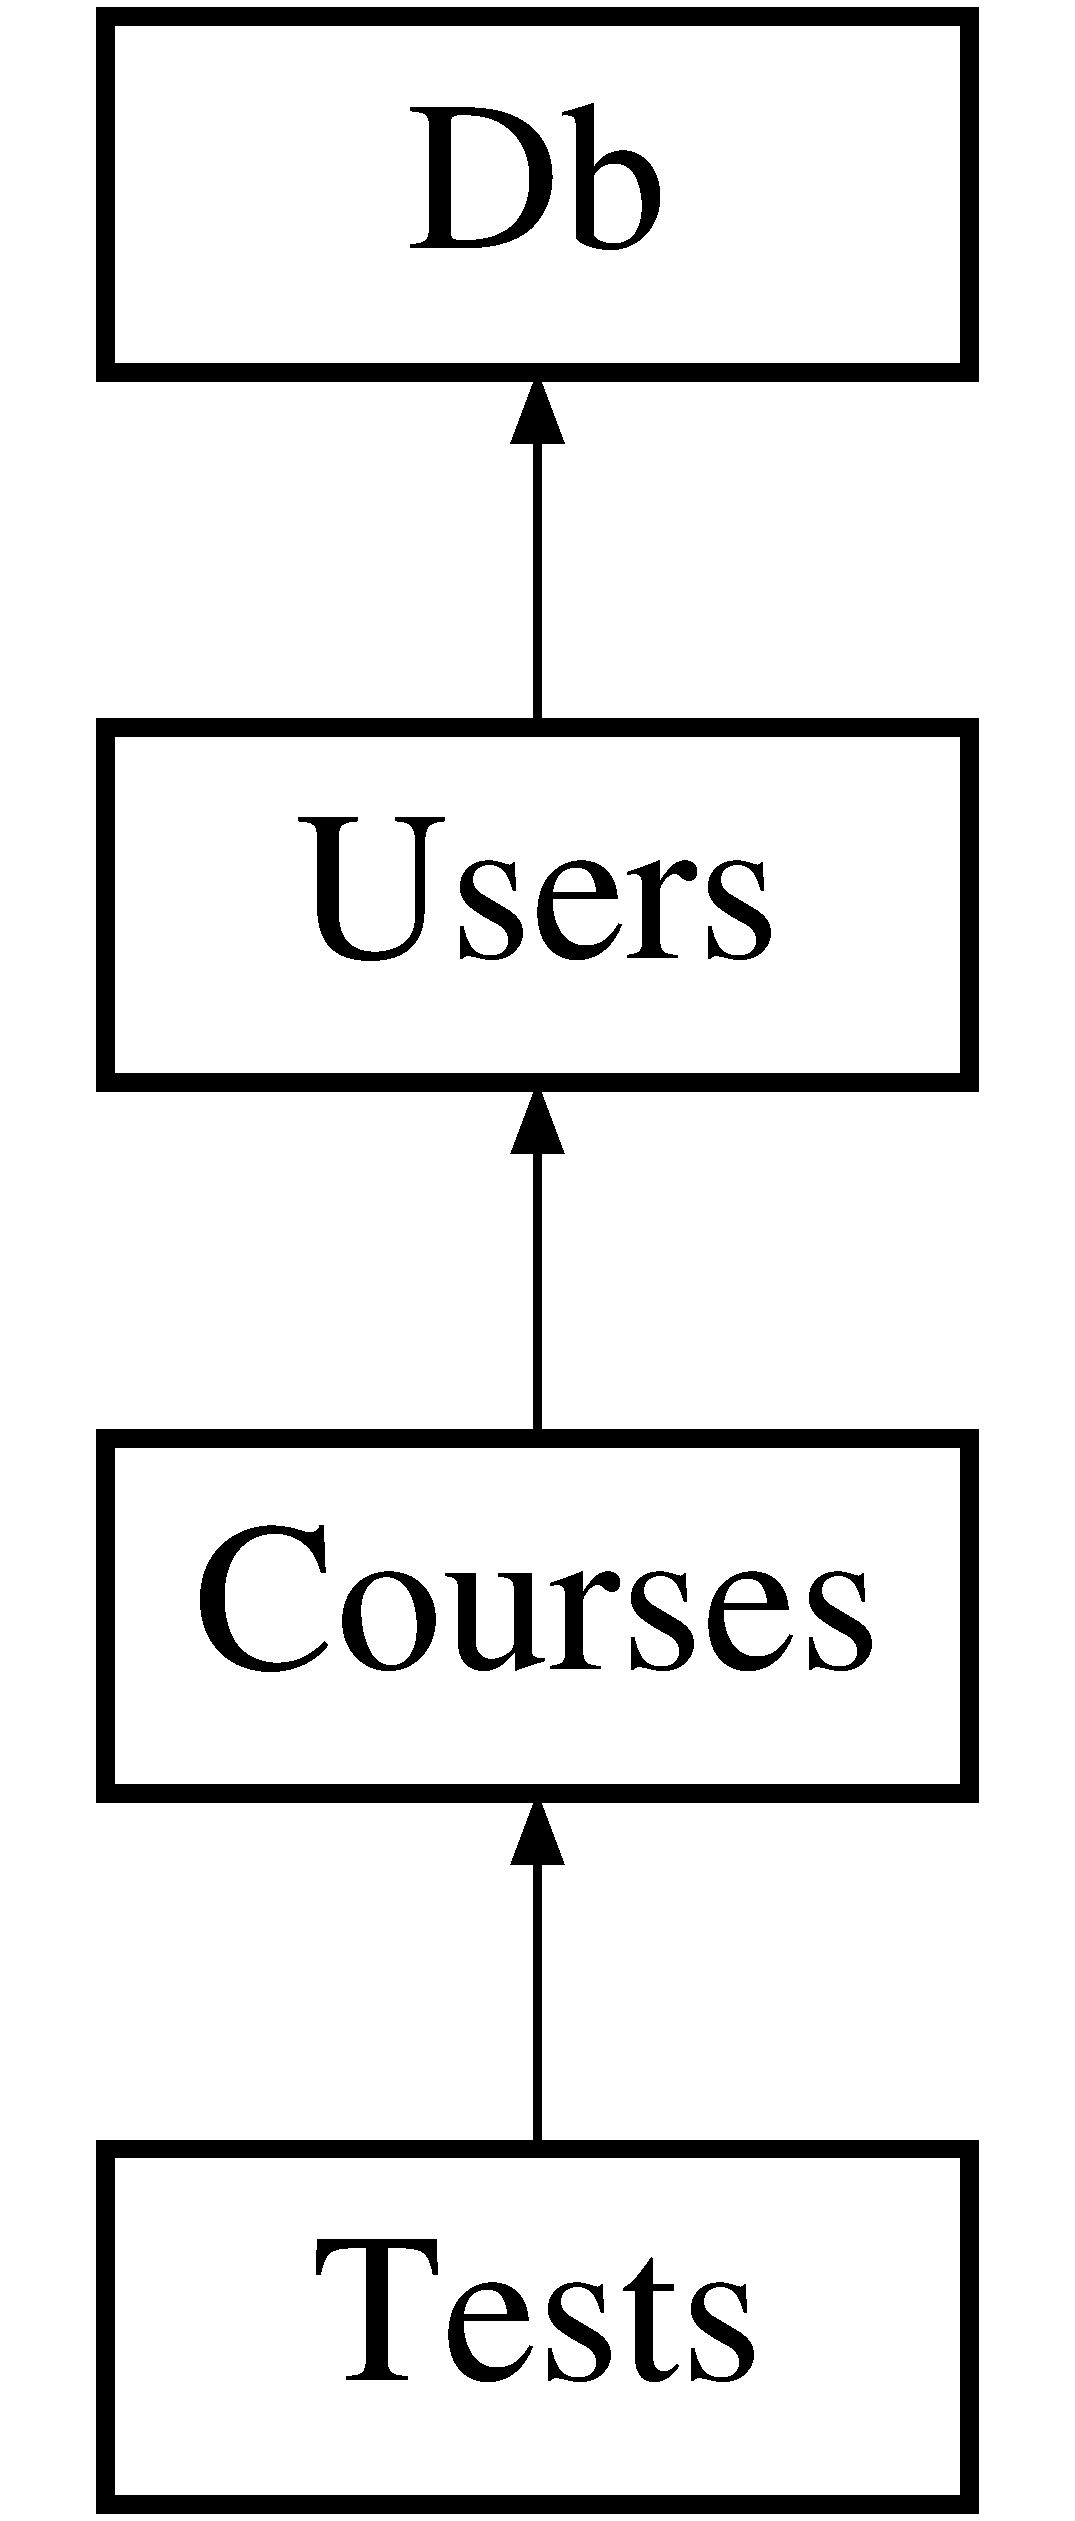
\includegraphics[height=4.000000cm]{class_courses}
\end{center}
\end{figure}
\subsection*{Public Member Functions}
\begin{DoxyCompactItemize}
\item 
\hyperlink{class_courses_a095c5d389db211932136b53f25f39685}{\-\_\-\-\_\-construct} ()
\item 
\hyperlink{class_courses_af008f367d5ca054454dacc1e8830d7fd}{fetch\-All} ()
\item 
\hyperlink{class_courses_a3e28346ce841ca962f8cd02bcf779f7e}{fetch\-By\-Id} (\$id)
\item 
\hyperlink{class_courses_a18c66bbad45c916eedc9dd9eaafdf2fe}{fetch\-By\-Name} (\$course\-Name)
\item 
\hyperlink{class_courses_a70e4ca7ed00c214b53247f1c58db0518}{create} (\$course\-Name, \$id, \$description)
\item 
\hyperlink{class_courses_a39bdae60b28491388b7526c4b2eefc7d}{modify} (\$id, \$column, \$value)
\item 
\hyperlink{class_courses_a523911d67549a199d2f019eec9cadf09}{add\-Instructor} (\$course\-Id, \$user\-Name)
\item 
\hyperlink{class_courses_a6704e97dc8543f819f8b1c14f4096ec0}{add\-Student} (\$course\-Id, \$user\-Name)
\item 
\hyperlink{class_courses_a180ac61277d5b0b6bb5d0d9c04b9ea1a}{course\-Exists} (\$course\-Id)
\item 
\hyperlink{class_courses_ade84f64416077da444e6fdda6d6f6265}{fetch\-Enrolled\-Courses} (\$user\-Name)
\end{DoxyCompactItemize}
\subsection*{Protected Attributes}
\begin{DoxyCompactItemize}
\item 
\hypertarget{class_courses_a0d9c79b9b86b3f5891c6d3892f12c6a0}{{\bfseries \$connection} = null}\label{class_courses_a0d9c79b9b86b3f5891c6d3892f12c6a0}

\end{DoxyCompactItemize}
\subsection*{Additional Inherited Members}


\subsection{Detailed Description}
This file manages all things related to courses  \hyperlink{class_db_a095c5d389db211932136b53f25f39685}{Db\-::\-\_\-\-\_\-construct()}  Users\-::\-\_\-\-\_\-construct() \begin{DoxyRefDesc}{Todo}
\item[\hyperlink{todo__todo000008}{Todo}]make a function to check if a course already exists \end{DoxyRefDesc}


\subsection{Constructor \& Destructor Documentation}
\hypertarget{class_courses_a095c5d389db211932136b53f25f39685}{\index{Courses@{Courses}!\-\_\-\-\_\-construct@{\-\_\-\-\_\-construct}}
\index{\-\_\-\-\_\-construct@{\-\_\-\-\_\-construct}!Courses@{Courses}}
\subsubsection[{\-\_\-\-\_\-construct}]{\setlength{\rightskip}{0pt plus 5cm}\-\_\-\-\_\-construct (
\begin{DoxyParamCaption}
{}
\end{DoxyParamCaption}
)}}\label{class_courses_a095c5d389db211932136b53f25f39685}
Constructor!  Users\-::\-\_\-\-\_\-construct() 

\subsection{Member Function Documentation}
\hypertarget{class_courses_a523911d67549a199d2f019eec9cadf09}{\index{Courses@{Courses}!add\-Instructor@{add\-Instructor}}
\index{add\-Instructor@{add\-Instructor}!Courses@{Courses}}
\subsubsection[{add\-Instructor}]{\setlength{\rightskip}{0pt plus 5cm}add\-Instructor (
\begin{DoxyParamCaption}
\item[{}]{\$course\-Id, }
\item[{}]{\$user\-Name}
\end{DoxyParamCaption}
)}}\label{class_courses_a523911d67549a199d2f019eec9cadf09}
This function adds an instructor and assigns them to a course


\begin{DoxyParams}[1]{Parameters}
string & {\em \$course\-Id} & The course id to add the user to \\
\hline
string & {\em \$user\-Name} & The user\-Name to be associated with the course\\
\hline
\end{DoxyParams}
\begin{DoxyReturn}{Returns}
boolean Returns true if successful, false if otherwise 
\end{DoxyReturn}
\hypertarget{class_courses_a6704e97dc8543f819f8b1c14f4096ec0}{\index{Courses@{Courses}!add\-Student@{add\-Student}}
\index{add\-Student@{add\-Student}!Courses@{Courses}}
\subsubsection[{add\-Student}]{\setlength{\rightskip}{0pt plus 5cm}add\-Student (
\begin{DoxyParamCaption}
\item[{}]{\$course\-Id, }
\item[{}]{\$user\-Name}
\end{DoxyParamCaption}
)}}\label{class_courses_a6704e97dc8543f819f8b1c14f4096ec0}
Add a student to a course


\begin{DoxyParams}{Parameters}
{\em \$course\-Id} & string the course to add a student to \\
\hline
{\em \$user\-Name} & string the username of the student to add\\
\hline
\end{DoxyParams}
\begin{DoxyReturn}{Returns}
boolean returns true if successful, false if otherwise 
\end{DoxyReturn}
\hypertarget{class_courses_a180ac61277d5b0b6bb5d0d9c04b9ea1a}{\index{Courses@{Courses}!course\-Exists@{course\-Exists}}
\index{course\-Exists@{course\-Exists}!Courses@{Courses}}
\subsubsection[{course\-Exists}]{\setlength{\rightskip}{0pt plus 5cm}course\-Exists (
\begin{DoxyParamCaption}
\item[{}]{\$course\-Id}
\end{DoxyParamCaption}
)}}\label{class_courses_a180ac61277d5b0b6bb5d0d9c04b9ea1a}
Checks whether a course exists in the database


\begin{DoxyParams}{Parameters}
{\em \$course\-Id} & string the id of the course to check\\
\hline
\end{DoxyParams}
\begin{DoxyReturn}{Returns}
boolean returns true if course exists, false otherwise 
\end{DoxyReturn}
\hypertarget{class_courses_a70e4ca7ed00c214b53247f1c58db0518}{\index{Courses@{Courses}!create@{create}}
\index{create@{create}!Courses@{Courses}}
\subsubsection[{create}]{\setlength{\rightskip}{0pt plus 5cm}create (
\begin{DoxyParamCaption}
\item[{}]{\$course\-Name, }
\item[{}]{\$id, }
\item[{}]{\$description}
\end{DoxyParamCaption}
)}}\label{class_courses_a70e4ca7ed00c214b53247f1c58db0518}
This function will create a course. Dies on an sql error


\begin{DoxyParams}[1]{Parameters}
string & {\em \$course\-Name} & \\
\hline
string & {\em \$id} & \\
\hline
string & {\em \$description} & \\
\hline
\end{DoxyParams}
\begin{DoxyReturn}{Returns}
boolean Return true if successful, or false if not 
\end{DoxyReturn}
\hypertarget{class_courses_af008f367d5ca054454dacc1e8830d7fd}{\index{Courses@{Courses}!fetch\-All@{fetch\-All}}
\index{fetch\-All@{fetch\-All}!Courses@{Courses}}
\subsubsection[{fetch\-All}]{\setlength{\rightskip}{0pt plus 5cm}fetch\-All (
\begin{DoxyParamCaption}
{}
\end{DoxyParamCaption}
)}}\label{class_courses_af008f367d5ca054454dacc1e8830d7fd}
This returns all courses in the database \begin{DoxyReturn}{Returns}
array$\vert$boolean Return an array that has both keyed and non-\/keyed values or false if the row was not found 
\end{DoxyReturn}
\hypertarget{class_courses_a3e28346ce841ca962f8cd02bcf779f7e}{\index{Courses@{Courses}!fetch\-By\-Id@{fetch\-By\-Id}}
\index{fetch\-By\-Id@{fetch\-By\-Id}!Courses@{Courses}}
\subsubsection[{fetch\-By\-Id}]{\setlength{\rightskip}{0pt plus 5cm}fetch\-By\-Id (
\begin{DoxyParamCaption}
\item[{}]{\$id}
\end{DoxyParamCaption}
)}}\label{class_courses_a3e28346ce841ca962f8cd02bcf779f7e}
This function returns a course according to its I\-D. Dies if no arguments are supplied or if an S\-Q\-L error is encountered


\begin{DoxyParams}[1]{Parameters}
string & {\em \$id} & The course id being searched for\\
\hline
\end{DoxyParams}
\begin{DoxyReturn}{Returns}
array$\vert$boolean Return an array that has both keyed and non-\/keyed values or false if the row was not found 
\end{DoxyReturn}
\hypertarget{class_courses_a18c66bbad45c916eedc9dd9eaafdf2fe}{\index{Courses@{Courses}!fetch\-By\-Name@{fetch\-By\-Name}}
\index{fetch\-By\-Name@{fetch\-By\-Name}!Courses@{Courses}}
\subsubsection[{fetch\-By\-Name}]{\setlength{\rightskip}{0pt plus 5cm}fetch\-By\-Name (
\begin{DoxyParamCaption}
\item[{}]{\$course\-Name}
\end{DoxyParamCaption}
)}}\label{class_courses_a18c66bbad45c916eedc9dd9eaafdf2fe}
This function returns a course according to its course name


\begin{DoxyParams}[1]{Parameters}
string & {\em \$course\-Name} & The course name being searched\\
\hline
\end{DoxyParams}
\begin{DoxyReturn}{Returns}
array$\vert$boolean Return an array that has both keyed and non-\/keyed values or false if the row was not found 
\end{DoxyReturn}
\hypertarget{class_courses_ade84f64416077da444e6fdda6d6f6265}{\index{Courses@{Courses}!fetch\-Enrolled\-Courses@{fetch\-Enrolled\-Courses}}
\index{fetch\-Enrolled\-Courses@{fetch\-Enrolled\-Courses}!Courses@{Courses}}
\subsubsection[{fetch\-Enrolled\-Courses}]{\setlength{\rightskip}{0pt plus 5cm}fetch\-Enrolled\-Courses (
\begin{DoxyParamCaption}
\item[{}]{\$user\-Name}
\end{DoxyParamCaption}
)}}\label{class_courses_ade84f64416077da444e6fdda6d6f6265}

\begin{DoxyParams}{Parameters}
{\em \$user\-Name} & string the user name to search for\\
\hline
\end{DoxyParams}
\begin{DoxyReturn}{Returns}
array$\vert$bool Return an array of courses if enrolled in any, false if otherwise 
\end{DoxyReturn}
\hypertarget{class_courses_a39bdae60b28491388b7526c4b2eefc7d}{\index{Courses@{Courses}!modify@{modify}}
\index{modify@{modify}!Courses@{Courses}}
\subsubsection[{modify}]{\setlength{\rightskip}{0pt plus 5cm}modify (
\begin{DoxyParamCaption}
\item[{}]{\$id, }
\item[{}]{\$column, }
\item[{}]{\$value}
\end{DoxyParamCaption}
)}}\label{class_courses_a39bdae60b28491388b7526c4b2eefc7d}
This function will change a selected column of the \hyperlink{class_courses}{Courses} table for a selected course id


\begin{DoxyParams}[1]{Parameters}
string & {\em \$id} & The id of the course to change \\
\hline
string & {\em \$column} & The column whose value will be changed \\
\hline
string & {\em \$value} & The value that will be inserted\\
\hline
\end{DoxyParams}
\begin{DoxyReturn}{Returns}
boolean Returns true if successful, otherwise false 
\end{DoxyReturn}


The documentation for this class was generated from the following file\-:\begin{DoxyCompactItemize}
\item 
requires/Courses.\-php\end{DoxyCompactItemize}

\hypertarget{class_db}{\section{Db Class Reference}
\label{class_db}\index{Db@{Db}}
}
Inheritance diagram for Db\-:\begin{figure}[H]
\begin{center}
\leavevmode
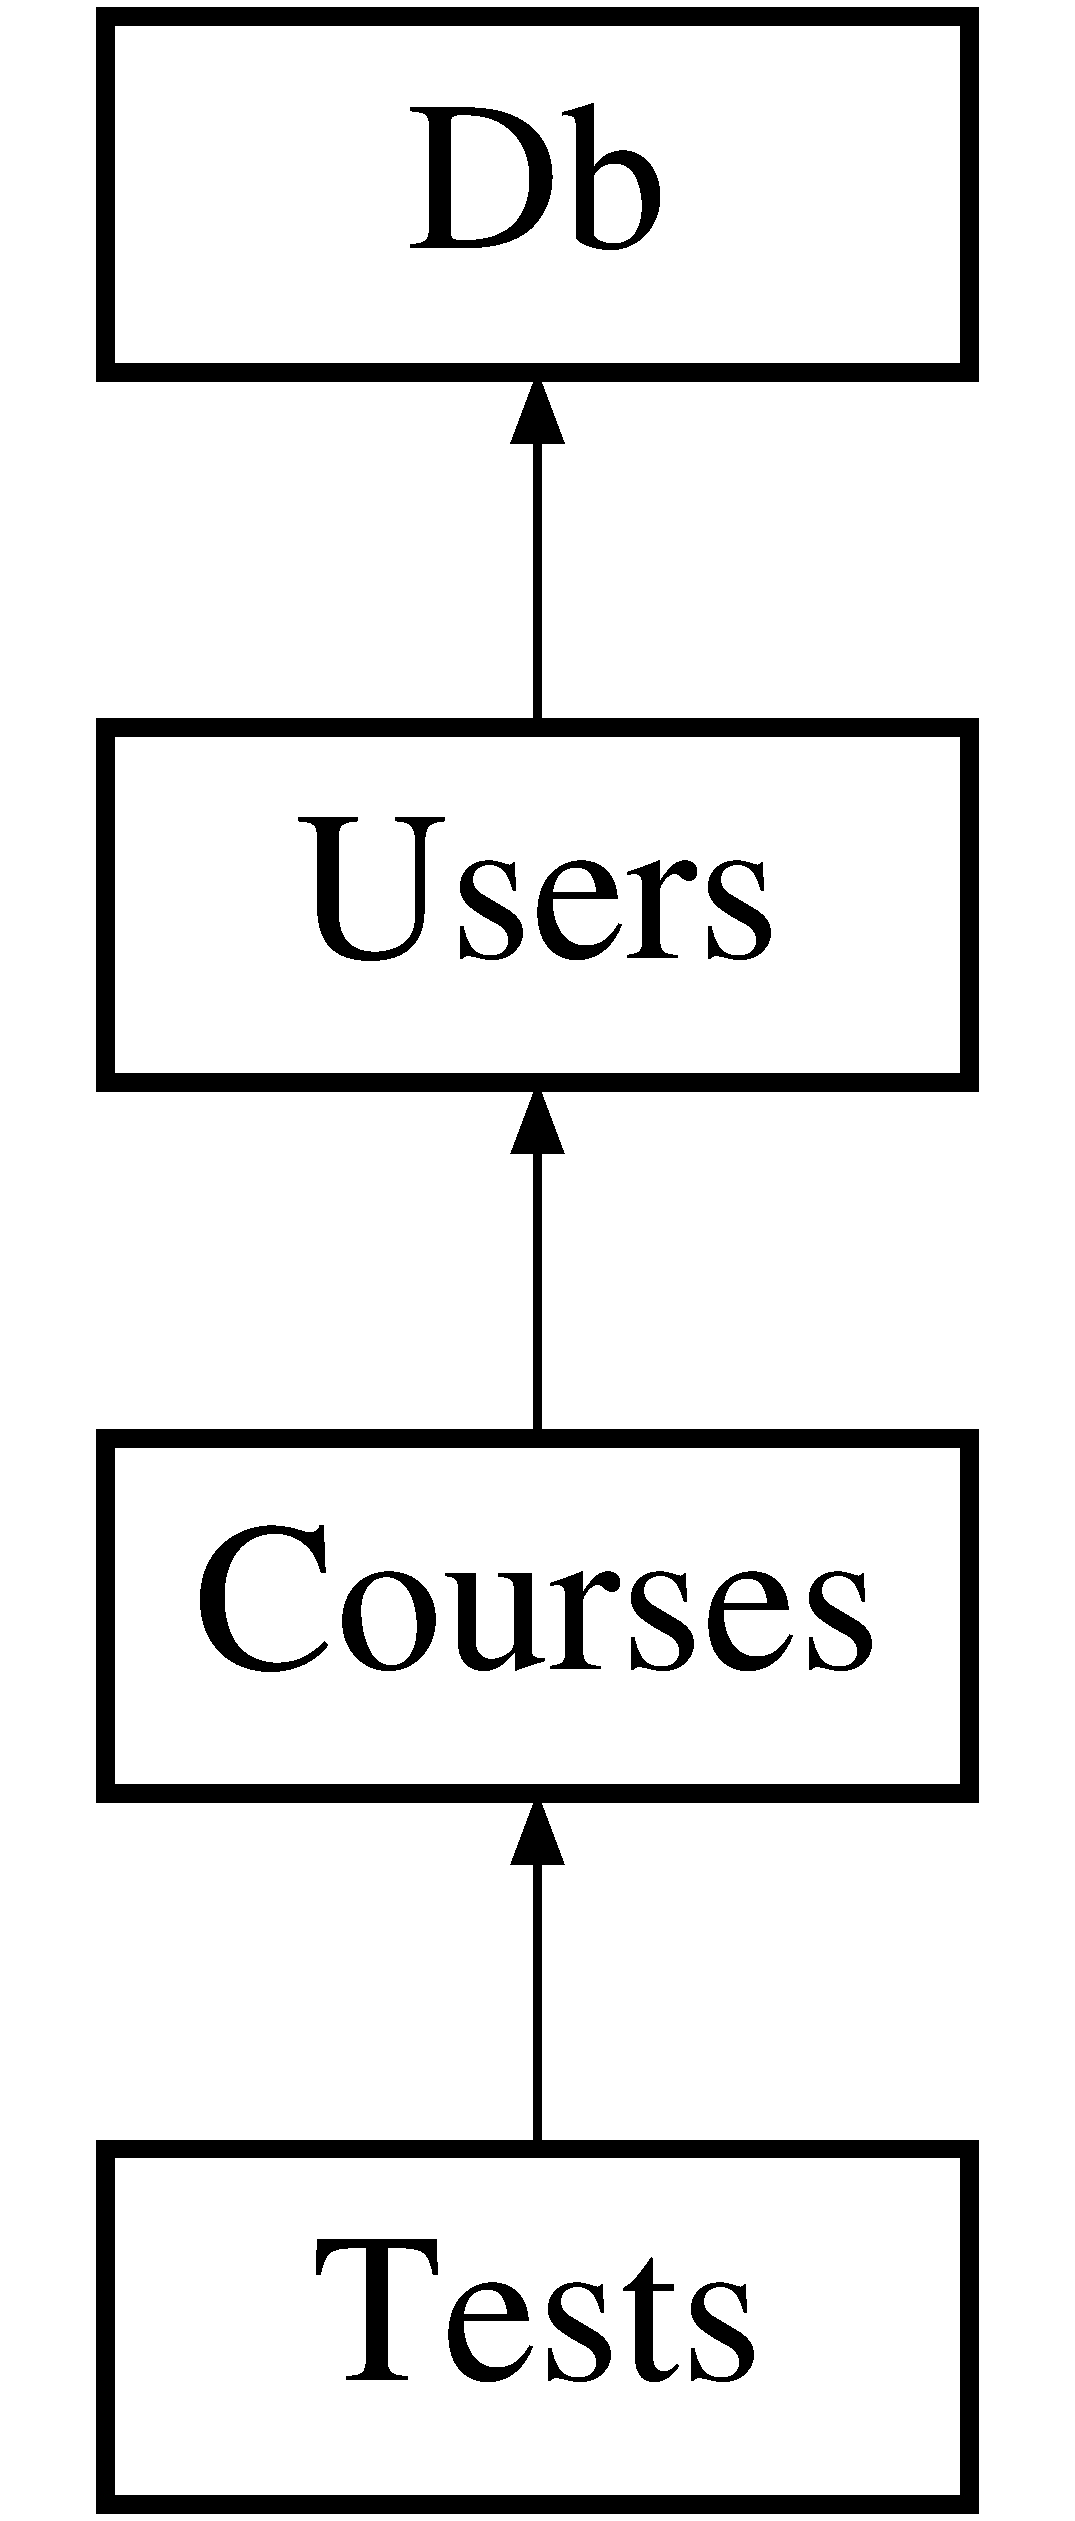
\includegraphics[height=4.000000cm]{class_db}
\end{center}
\end{figure}
\subsection*{Public Member Functions}
\begin{DoxyCompactItemize}
\item 
\hyperlink{class_db_a095c5d389db211932136b53f25f39685}{\-\_\-\-\_\-construct} ()
\item 
\hyperlink{class_db_a78572828d11dcdf2a498497d9001d557}{connect} ()
\item 
\hyperlink{class_db_aa69c8bf1f1dcf4e72552efff1fe3e87e}{close} ()
\item 
\hyperlink{class_db_a7fa48f6882eccec91ea9c433e1ad2a57}{connection} ()
\item 
\hyperlink{class_db_a528ec08d78133851fec5e71ed9cf3779}{fetch\-All\-Rows} (\$sql\-Result)
\item 
\hypertarget{class_db_a79f742455432acb343b7ebed6013995f}{{\bfseries check\-Sql\-Result} (\$sql\-Result)}\label{class_db_a79f742455432acb343b7ebed6013995f}

\end{DoxyCompactItemize}
\subsection*{Data Fields}
\begin{DoxyCompactItemize}
\item 
\hypertarget{class_db_a3d332a3c374a53802495dcb045f6133f}{{\bfseries \$tables}}\label{class_db_a3d332a3c374a53802495dcb045f6133f}

\end{DoxyCompactItemize}
\subsection*{Protected Attributes}
\begin{DoxyCompactItemize}
\item 
\hypertarget{class_db_a7691c0162d89de0b6ba47edcd8ba8878}{{\bfseries \$database}}\label{class_db_a7691c0162d89de0b6ba47edcd8ba8878}

\item 
\hypertarget{class_db_a607686ef9f99ea7c42f4f3dd3dbb2b0d}{{\bfseries \$password}}\label{class_db_a607686ef9f99ea7c42f4f3dd3dbb2b0d}

\item 
\hypertarget{class_db_a711797613cb863ca0756df789c396bf2}{{\bfseries \$host}}\label{class_db_a711797613cb863ca0756df789c396bf2}

\item 
\hypertarget{class_db_a598ca4e71b15a1313ec95f0df1027ca5}{{\bfseries \$user}}\label{class_db_a598ca4e71b15a1313ec95f0df1027ca5}

\item 
\hypertarget{class_db_a0d9c79b9b86b3f5891c6d3892f12c6a0}{{\bfseries \$connection} = null}\label{class_db_a0d9c79b9b86b3f5891c6d3892f12c6a0}

\end{DoxyCompactItemize}


\subsection{Constructor \& Destructor Documentation}
\hypertarget{class_db_a095c5d389db211932136b53f25f39685}{\index{Db@{Db}!\-\_\-\-\_\-construct@{\-\_\-\-\_\-construct}}
\index{\-\_\-\-\_\-construct@{\-\_\-\-\_\-construct}!Db@{Db}}
\subsubsection[{\-\_\-\-\_\-construct}]{\setlength{\rightskip}{0pt plus 5cm}\-\_\-\-\_\-construct (
\begin{DoxyParamCaption}
{}
\end{DoxyParamCaption}
)}}\label{class_db_a095c5d389db211932136b53f25f39685}
Constructor method. First checks for a user-\/config.\-ini file, then a default-\/config.\-ini file if the user-\/config.\-ini file is not found. If both are not found, throw an error


\begin{DoxyExceptions}{Exceptions}
{\em error} & Complains that configuration file is not found and halts execution \\
\hline
\end{DoxyExceptions}


\subsection{Member Function Documentation}
\hypertarget{class_db_aa69c8bf1f1dcf4e72552efff1fe3e87e}{\index{Db@{Db}!close@{close}}
\index{close@{close}!Db@{Db}}
\subsubsection[{close}]{\setlength{\rightskip}{0pt plus 5cm}close (
\begin{DoxyParamCaption}
{}
\end{DoxyParamCaption}
)}}\label{class_db_aa69c8bf1f1dcf4e72552efff1fe3e87e}
Closes the connection. Dies if it fails \hypertarget{class_db_a78572828d11dcdf2a498497d9001d557}{\index{Db@{Db}!connect@{connect}}
\index{connect@{connect}!Db@{Db}}
\subsubsection[{connect}]{\setlength{\rightskip}{0pt plus 5cm}connect (
\begin{DoxyParamCaption}
{}
\end{DoxyParamCaption}
)}}\label{class_db_a78572828d11dcdf2a498497d9001d557}
Connects to the database. Dies if it fails \hypertarget{class_db_a7fa48f6882eccec91ea9c433e1ad2a57}{\index{Db@{Db}!connection@{connection}}
\index{connection@{connection}!Db@{Db}}
\subsubsection[{connection}]{\setlength{\rightskip}{0pt plus 5cm}connection (
\begin{DoxyParamCaption}
{}
\end{DoxyParamCaption}
)}}\label{class_db_a7fa48f6882eccec91ea9c433e1ad2a57}
Connection accessor \begin{DoxyReturn}{Returns}
object My\-S\-Q\-Li connection object 
\end{DoxyReturn}
\hypertarget{class_db_a528ec08d78133851fec5e71ed9cf3779}{\index{Db@{Db}!fetch\-All\-Rows@{fetch\-All\-Rows}}
\index{fetch\-All\-Rows@{fetch\-All\-Rows}!Db@{Db}}
\subsubsection[{fetch\-All\-Rows}]{\setlength{\rightskip}{0pt plus 5cm}fetch\-All\-Rows (
\begin{DoxyParamCaption}
\item[{}]{\$sql\-Result}
\end{DoxyParamCaption}
)}}\label{class_db_a528ec08d78133851fec5e71ed9cf3779}

\begin{DoxyParams}{Parameters}
{\em \$sql\-Result} & object The result of an S\-Q\-L query to get rows from\\
\hline
\end{DoxyParams}
\begin{DoxyReturn}{Returns}
array The resultant rows from the S\-Q\-L query 
\end{DoxyReturn}


The documentation for this class was generated from the following file\-:\begin{DoxyCompactItemize}
\item 
requires/Db.\-php\end{DoxyCompactItemize}

\hypertarget{class_tests}{\section{Tests Class Reference}
\label{class_tests}\index{Tests@{Tests}}
}
Inheritance diagram for Tests\-:\begin{figure}[H]
\begin{center}
\leavevmode
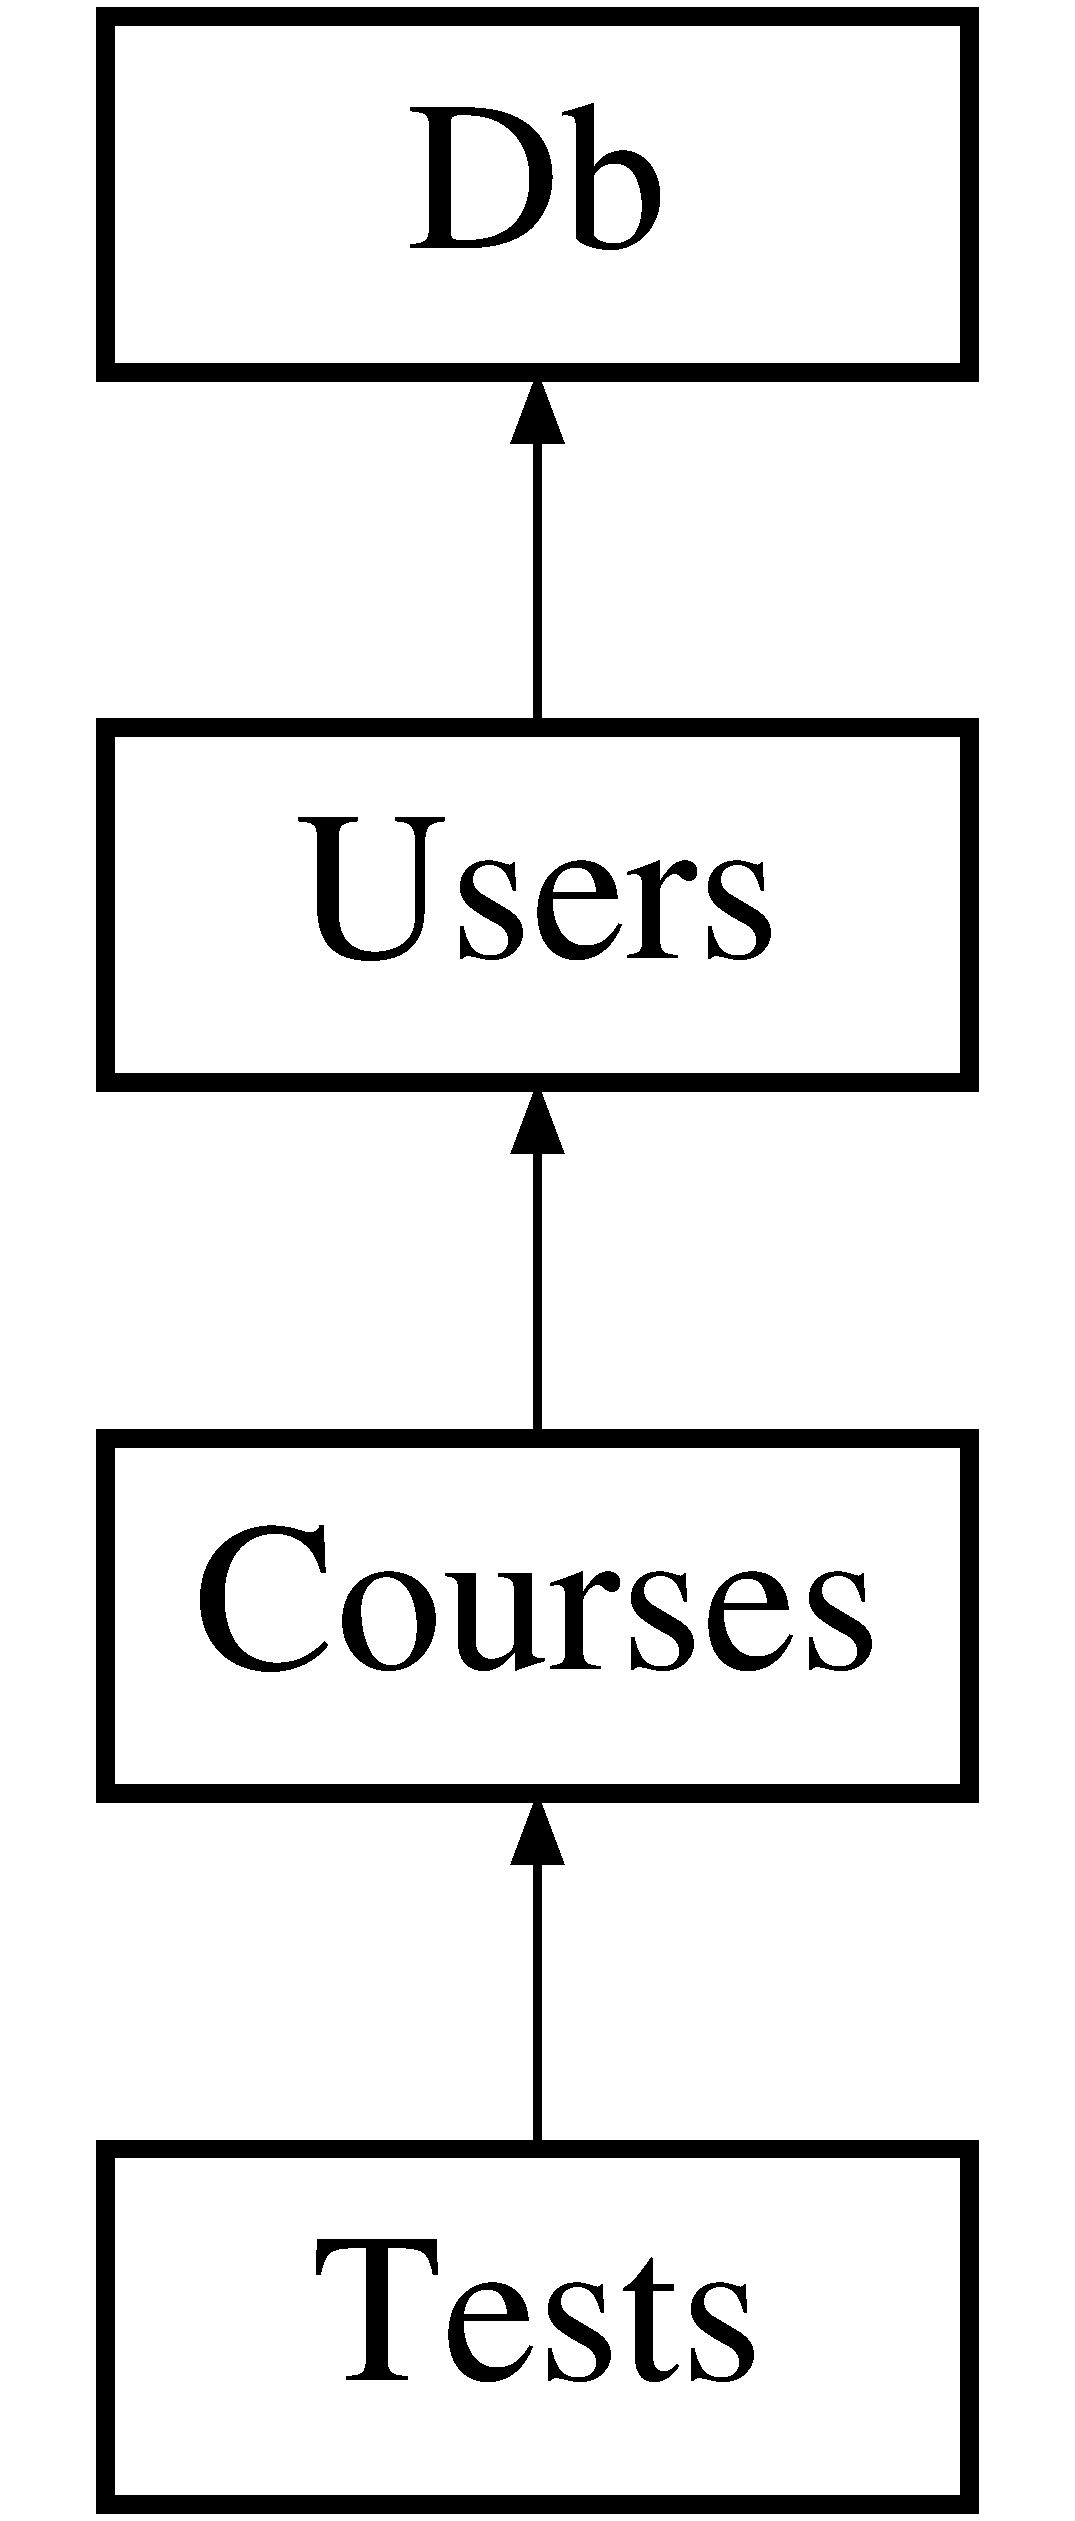
\includegraphics[height=4.000000cm]{class_tests}
\end{center}
\end{figure}
\subsection*{Public Member Functions}
\begin{DoxyCompactItemize}
\item 
\hyperlink{class_tests_a095c5d389db211932136b53f25f39685}{\-\_\-\-\_\-construct} ()
\item 
\hyperlink{class_tests_a72da384132fd1eb42dfad51c052ca553}{make\-Test} (\$data)
\item 
\hyperlink{class_tests_a615e2a92a28b88696873320d56041cde}{update\-Test} (\$data)
\item 
\hypertarget{class_tests_a7803b46e1b0460768e4f12c9abcf41a1}{{\bfseries fetch\-By\-Name} (\$name)}\label{class_tests_a7803b46e1b0460768e4f12c9abcf41a1}

\item 
\hypertarget{class_tests_a36f36c993f4da045e541d3b8818a2734}{{\bfseries list\-All} ()}\label{class_tests_a36f36c993f4da045e541d3b8818a2734}

\end{DoxyCompactItemize}
\subsection*{Protected Attributes}
\begin{DoxyCompactItemize}
\item 
\hypertarget{class_tests_a0d9c79b9b86b3f5891c6d3892f12c6a0}{{\bfseries \$connection}}\label{class_tests_a0d9c79b9b86b3f5891c6d3892f12c6a0}

\end{DoxyCompactItemize}
\subsection*{Additional Inherited Members}


\subsection{Constructor \& Destructor Documentation}
\hypertarget{class_tests_a095c5d389db211932136b53f25f39685}{\index{Tests@{Tests}!\-\_\-\-\_\-construct@{\-\_\-\-\_\-construct}}
\index{\-\_\-\-\_\-construct@{\-\_\-\-\_\-construct}!Tests@{Tests}}
\subsubsection[{\-\_\-\-\_\-construct}]{\setlength{\rightskip}{0pt plus 5cm}\-\_\-\-\_\-construct (
\begin{DoxyParamCaption}
{}
\end{DoxyParamCaption}
)}}\label{class_tests_a095c5d389db211932136b53f25f39685}
Constructor!  \hyperlink{class_courses_a095c5d389db211932136b53f25f39685}{Courses\-::\-\_\-\-\_\-construct()} 

\subsection{Member Function Documentation}
\hypertarget{class_tests_a72da384132fd1eb42dfad51c052ca553}{\index{Tests@{Tests}!make\-Test@{make\-Test}}
\index{make\-Test@{make\-Test}!Tests@{Tests}}
\subsubsection[{make\-Test}]{\setlength{\rightskip}{0pt plus 5cm}make\-Test (
\begin{DoxyParamCaption}
\item[{}]{\$data}
\end{DoxyParamCaption}
)}}\label{class_tests_a72da384132fd1eb42dfad51c052ca553}
This function will make a test if it does not exist, or update a current test if it exists


\begin{DoxyParams}{Parameters}
{\em \$data} & array Takes in an array of the test\\
\hline
\end{DoxyParams}
\begin{DoxyReturn}{Returns}
bool True if successful, false if it fails 
\end{DoxyReturn}
\hypertarget{class_tests_a615e2a92a28b88696873320d56041cde}{\index{Tests@{Tests}!update\-Test@{update\-Test}}
\index{update\-Test@{update\-Test}!Tests@{Tests}}
\subsubsection[{update\-Test}]{\setlength{\rightskip}{0pt plus 5cm}update\-Test (
\begin{DoxyParamCaption}
\item[{}]{\$data}
\end{DoxyParamCaption}
)}}\label{class_tests_a615e2a92a28b88696873320d56041cde}

\begin{DoxyParams}{Parameters}
{\em \$data} & array Takes in an array of the test\\
\hline
\end{DoxyParams}
\begin{DoxyReturn}{Returns}
bool Returns true if successful, false if otherwise. Will fail with an error if input is incorrect 
\end{DoxyReturn}


The documentation for this class was generated from the following file\-:\begin{DoxyCompactItemize}
\item 
requires/Tests.\-php\end{DoxyCompactItemize}

\hypertarget{class_users}{\section{Users Class Reference}
\label{class_users}\index{Users@{Users}}
}
Inheritance diagram for Users\-:\begin{figure}[H]
\begin{center}
\leavevmode
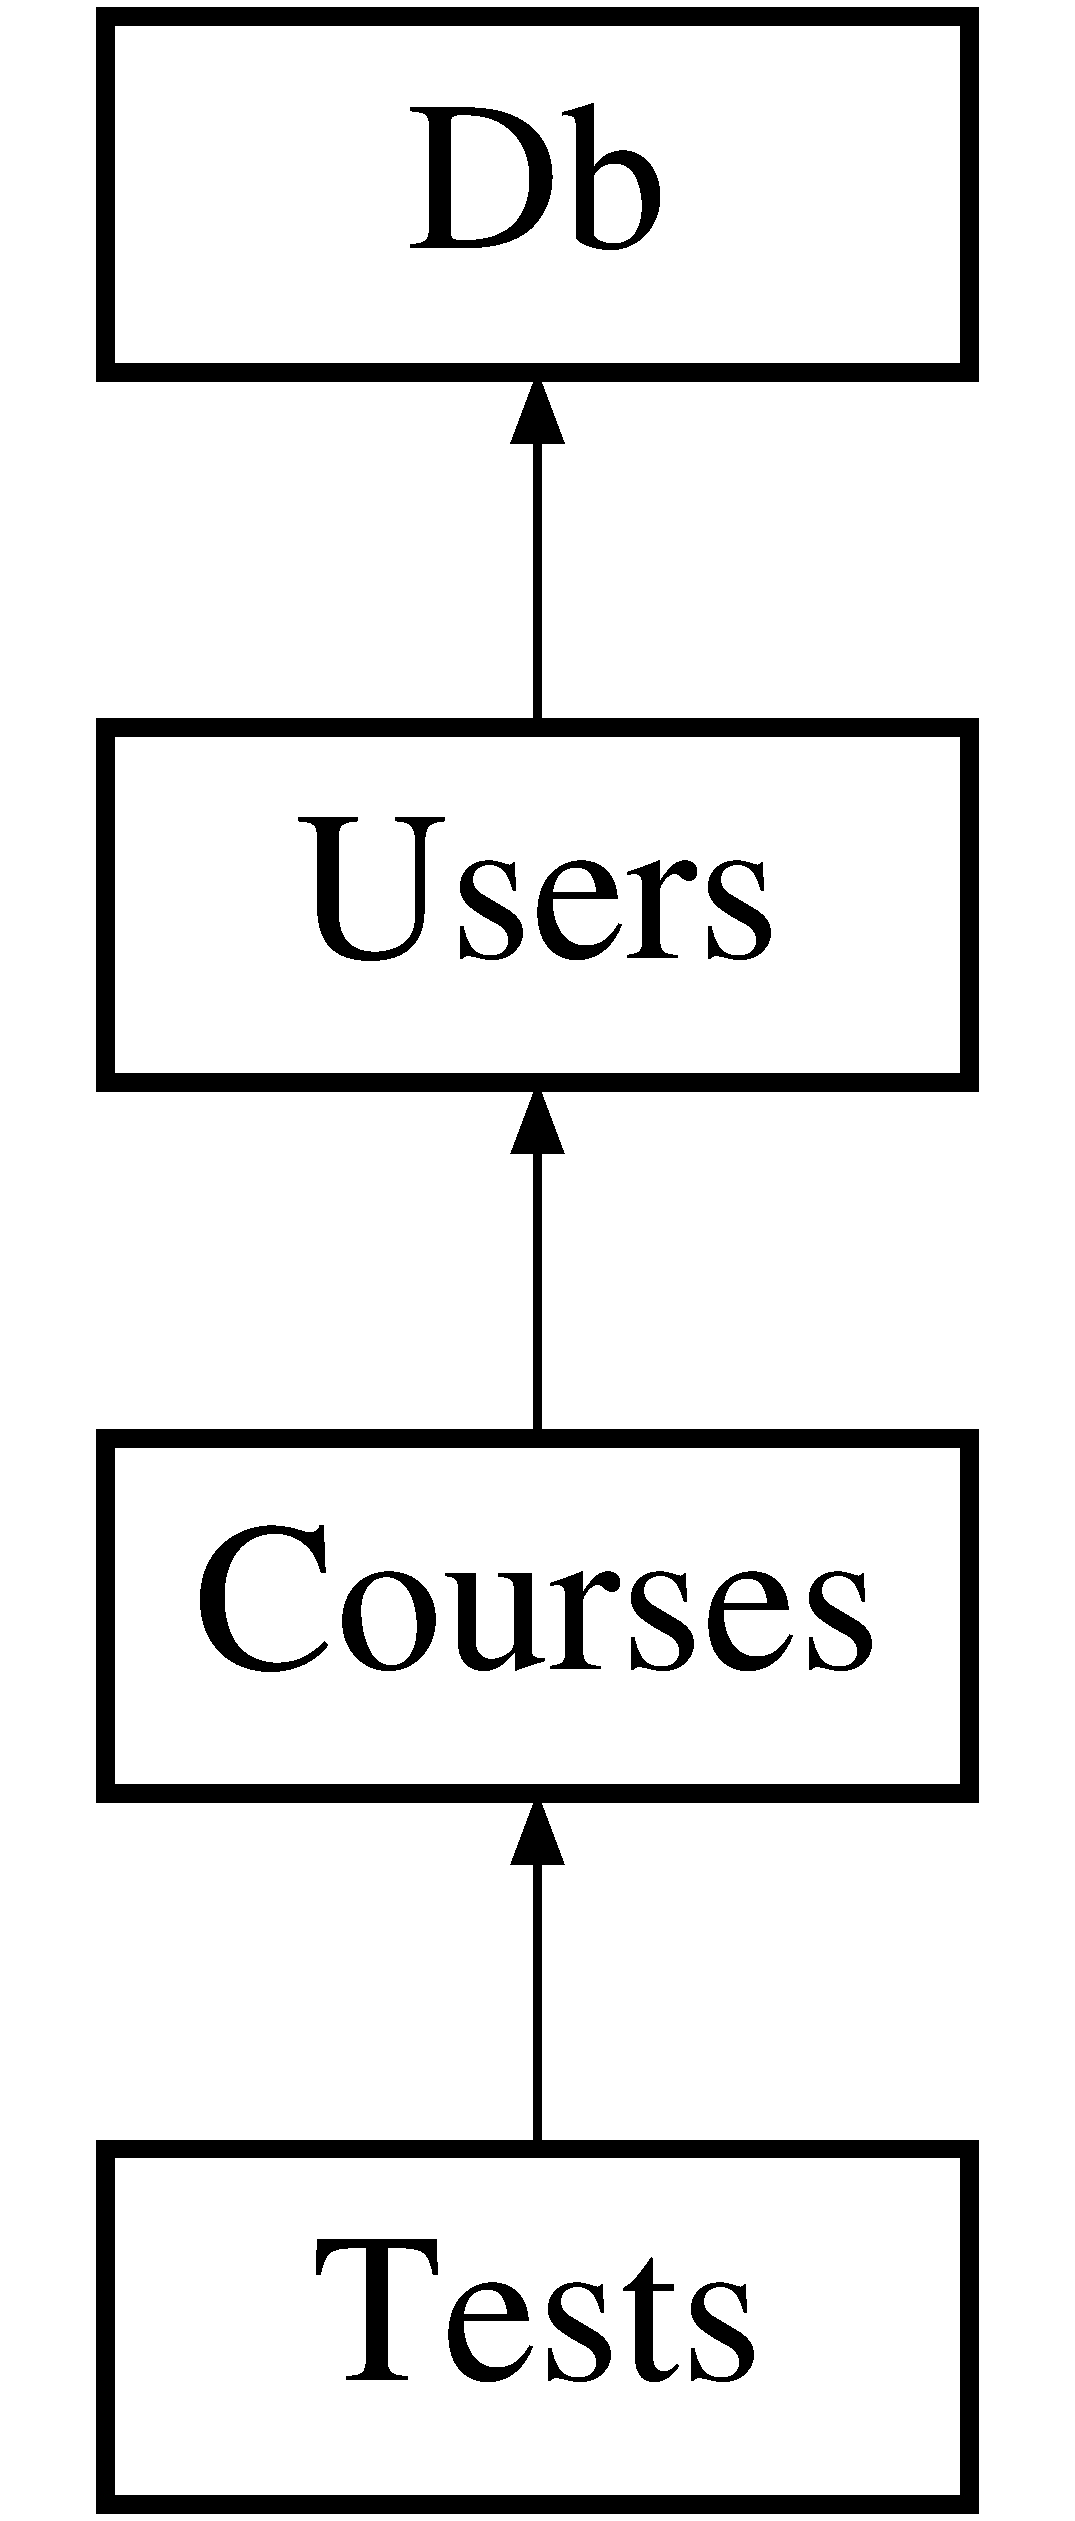
\includegraphics[height=4.000000cm]{class_users}
\end{center}
\end{figure}
\subsection*{Public Member Functions}
\begin{DoxyCompactItemize}
\item 
\hyperlink{class_users_a8fe0db35ee8e4bf70ab574b3d0d3cfd0}{check\-String} (\$string)
\item 
\hyperlink{class_users_a03f071927e9f1a1a1930622153ca76fa}{user\-Exists} (\$user\-Name)
\item 
\hyperlink{class_users_a7b27bffdb6648e9f5479b7bcbaf8a5e6}{check\-Password} (\$user\-Name, \$password)
\item 
\hyperlink{class_users_aac93d8c8a65d6be245c8243b85175b64}{fetch\-User} (\$user\-Name)
\item 
\hyperlink{class_users_a9ef91bc8e5330e06661bd8fc95ea98b3}{create} (\$user\-Name, \$password)
\end{DoxyCompactItemize}
\subsection*{Protected Attributes}
\begin{DoxyCompactItemize}
\item 
\hypertarget{class_users_a0d9c79b9b86b3f5891c6d3892f12c6a0}{{\bfseries \$connection} = null}\label{class_users_a0d9c79b9b86b3f5891c6d3892f12c6a0}

\end{DoxyCompactItemize}
\subsection*{Additional Inherited Members}


\subsection{Detailed Description}
This class contains methods to manipulate user data. Extends the \hyperlink{class_db}{Db} class  \hyperlink{class_db_a095c5d389db211932136b53f25f39685}{Db\-::\-\_\-\-\_\-construct()} 

\subsection{Member Function Documentation}
\hypertarget{class_users_a7b27bffdb6648e9f5479b7bcbaf8a5e6}{\index{Users@{Users}!check\-Password@{check\-Password}}
\index{check\-Password@{check\-Password}!Users@{Users}}
\subsubsection[{check\-Password}]{\setlength{\rightskip}{0pt plus 5cm}check\-Password (
\begin{DoxyParamCaption}
\item[{}]{\$user\-Name, }
\item[{}]{\$password}
\end{DoxyParamCaption}
)}}\label{class_users_a7b27bffdb6648e9f5479b7bcbaf8a5e6}
This function checks the user password against the one stored in the database


\begin{DoxyParams}[1]{Parameters}
string & {\em \$user\-Name} & The username associated with the password being checked \\
\hline
string & {\em \$password} & The password string being checked\\
\hline
\end{DoxyParams}
\begin{DoxyReturn}{Returns}
boolean Returns true if a match, false if it failed but did not produce an error 
\end{DoxyReturn}
\hypertarget{class_users_a8fe0db35ee8e4bf70ab574b3d0d3cfd0}{\index{Users@{Users}!check\-String@{check\-String}}
\index{check\-String@{check\-String}!Users@{Users}}
\subsubsection[{check\-String}]{\setlength{\rightskip}{0pt plus 5cm}check\-String (
\begin{DoxyParamCaption}
\item[{}]{\$string}
\end{DoxyParamCaption}
)}}\label{class_users_a8fe0db35ee8e4bf70ab574b3d0d3cfd0}
Simple method to check if the supplied argument is a string and has a length greater than zero


\begin{DoxyParams}[1]{Parameters}
string | array & {\em \$string} & the string or array containing strings to check\\
\hline
\end{DoxyParams}
\begin{DoxyReturn}{Returns}
boolean returns true if argument is a string and has a length greater than zero, false if otherwise 
\end{DoxyReturn}
\hypertarget{class_users_a9ef91bc8e5330e06661bd8fc95ea98b3}{\index{Users@{Users}!create@{create}}
\index{create@{create}!Users@{Users}}
\subsubsection[{create}]{\setlength{\rightskip}{0pt plus 5cm}create (
\begin{DoxyParamCaption}
\item[{}]{\$user\-Name, }
\item[{}]{\$password}
\end{DoxyParamCaption}
)}}\label{class_users_a9ef91bc8e5330e06661bd8fc95ea98b3}
This function handles user creation. The user will also have an auto-\/incremented numerical id associated with their account. This function M\-U\-S\-T have two arguments.


\begin{DoxyParams}[1]{Parameters}
string & {\em \$user\-Name} & The user\-Name that will be inserted into the table \\
\hline
string & {\em \$password} & The password that will be inserted into the table\\
\hline
\end{DoxyParams}
\begin{DoxyReturn}{Returns}
boolean Return true if creation succeeded, false if it failed but did not produce an error 
\end{DoxyReturn}
\hypertarget{class_users_aac93d8c8a65d6be245c8243b85175b64}{\index{Users@{Users}!fetch\-User@{fetch\-User}}
\index{fetch\-User@{fetch\-User}!Users@{Users}}
\subsubsection[{fetch\-User}]{\setlength{\rightskip}{0pt plus 5cm}fetch\-User (
\begin{DoxyParamCaption}
\item[{}]{\$user\-Name}
\end{DoxyParamCaption}
)}}\label{class_users_aac93d8c8a65d6be245c8243b85175b64}
This function retrieves a users's row as both a keyed and a non-\/keyed array


\begin{DoxyParams}[1]{Parameters}
string & {\em \$user\-Name} & The username whose row you want to fetch\\
\hline
\end{DoxyParams}
\begin{DoxyReturn}{Returns}
array$\vert$boolean Return an array that has both keyed and non-\/keyed values or false if the row was not found 
\end{DoxyReturn}
\hypertarget{class_users_a03f071927e9f1a1a1930622153ca76fa}{\index{Users@{Users}!user\-Exists@{user\-Exists}}
\index{user\-Exists@{user\-Exists}!Users@{Users}}
\subsubsection[{user\-Exists}]{\setlength{\rightskip}{0pt plus 5cm}user\-Exists (
\begin{DoxyParamCaption}
\item[{}]{\$user\-Name}
\end{DoxyParamCaption}
)}}\label{class_users_a03f071927e9f1a1a1930622153ca76fa}
This function checks if a user exists in the user table


\begin{DoxyParams}[1]{Parameters}
string & {\em \$user\-Name} & The user's name in the database\\
\hline
\end{DoxyParams}
\begin{DoxyReturn}{Returns}
boolean returns true if the operation completed successfully, false if it failed but did not produce an error 
\end{DoxyReturn}


The documentation for this class was generated from the following file\-:\begin{DoxyCompactItemize}
\item 
requires/Users.\-php\end{DoxyCompactItemize}

%--- End generated contents ---

% Index
\newpage
\phantomsection
\addcontentsline{toc}{chapter}{Index}
\printindex

\end{document}
